% !TeX document-id = {38ad272c-6b95-4178-b409-8ae7f3766667}
% !TeX spellcheck = en_US
% !TeX root = ../../build/architecture.tex
% !TeX TXS-program:compile = txs:///xelatex/[--shell-escape]


\renewcommand{\mytitle}{Ethereum Layer 1}
\ifZEROSEC \fi
\ifSEC \section{\mytitle{}}\fi
\ifSUBSEC \subsection{\mytitle{}}\fi
\ifSUBSUBSEC \subsubsection{\mytitle{}}\fi



\begin{frame}{Ethereum Layer 1}
\begin{figure}[H]
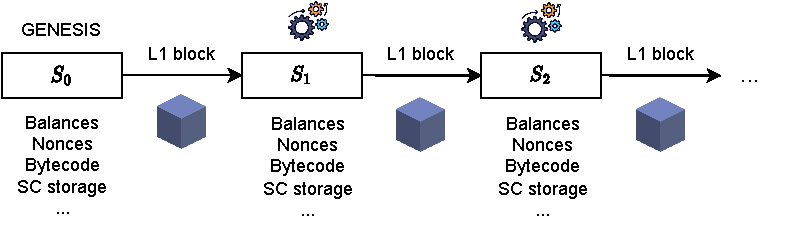
\includegraphics[width=0.8\columnwidth]{\zkevmdir/figures/concepts/layer1-ethereum/ethereum-layer1}
\end{figure}
\centering
Transactions in L1 blocks are \textbf{available} and \textbf{executed}.
\end{frame}




\begin{frame} {Representation of Each State}
  \begin{itemize}
    \item $S_i$ denotes a cryptographic summary of the data of state $i$.
    \item $S_i$ is implemented as the \textbf{root} of a Merkle Tree 
    that includes data items as leaves of the $i$-th state.
    \newline
    \begin{figure}[H]
      \centering
      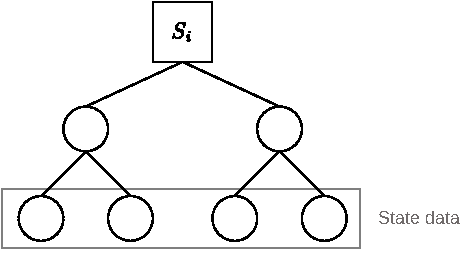
\includegraphics[width=0.4\columnwidth]{\zkevmdir/figures/concepts/layer1-ethereum/representation-state}
    \end{figure}
    % TODO Make figure smaller
  \end{itemize}
\end{frame}